\addtocontents{toc}{\protect\addvspace{5pt}}
\chapter{DASAR TEORI}

\section{Perambatan Gelombang Nonlinear Serat Optik}

Respons sistem komunikasi global mengalami perkembangan pesat pada tahun 1970, di mana laju atenuasi sinyal dapat diredam hingga 20 dB/km. Serat optik, kemudian, dapat digunakan sebagai media komunikasi secara luas. Penelitian atas serat optik berfokus terhadap nonlinearitas serat yang bertanggung jawab atas pembentukan soliton, pulsa gelombang khusus yang mampu mempertahankan bentuknya ketika merambat pada media nonlinear dengan ppenyebaran pulsa yang minimal \shortcite{abdillah2023soliton}. Perambatan gelombang pada serat optik dapat dinyatakan secara matematis dengan Persamaan Schr\"{o}dinger Nonlinear (NLS) yang dinyatakan sebagai berikut: 

\begin{equation}
    \label{mainNLSE}
    \frac{\partial A(t,z)}{\partial z}+\frac{\alpha}{2}A(t,z) + \left( \sum_{k=1}^n\beta_k \frac{i^{k-1}}{k!}\frac{\partial^k}{\partial T^k}\right)A - i \gamma |A|^2A(t,z) = 0
\end{equation}

Variabel \(A(t,z)\) menyatakan pulsa gelombang longitudinal kompleks sebagai fungsi waktu \(t\) dan posisi \(z\). Daya optis dari gelombang dapat dinyatakan dengan menormalisasi pulsa, \(|A|^2\). Parameter \(\alpha\) menyatakan atenuasi serat optik yang utamanya disebabkan oleh absorpsi material dan hamburan Rayleigh yang meningkat seiring dengan frekuensi gelombang transmisi. Koefisien \(\beta_n\) menyatakan dispersi ordo ke-$n$, dan koefisien $\gamma$ menyatakan indeks bias nonlinear serat optik \shortcite{MARTINS2024103636}. 

Dalam memodelkan perambatan pulsa, digunakan kerangka waktu bergerak ($t = t-\beta_1z$) yang mengikuti gerakan pulsa, sehingga faktor dispersi orde pertama $\beta_1$ diabaikan \shortcite{agrawal2019nonlinear}. Sementara itu, pada konteks perambatan pulsa \emph{ultrashort}, koefisien dispersi dibatasi hingga mencapai orde ketiga. Hal ini memberikan persamaan:

\begin{align}
    \label{usNLSE}
    \frac{\partial A(t,z)}{\partial z}
    &+ \frac{\alpha}{2} A(t,z) 
    + i \frac{\beta_2}{2} \frac{\partial^2 A(t,z)}{\partial t^2} \notag \\
    &-  \frac{\beta_3}{6} \frac{\partial^3 A(t,z)}{\partial t^3} 
    - i \gamma |A(t,z)|^2 A(t,z) 
    = 0
\end{align}

Dispersi kromatis terjadi oleh karena interaksi dari elektron terikat medium terhadap frekuensi gelombang. Dispersi orde kedua $\beta_2$ menyatakan dispersi kecepatan grup yang menentukan bagaimana perubahan kecepatan grup. Nilai $\beta_2$ negatif menunjukkan bahwa gelombang berfrekuensi tinggi merambat lebih cepat daripada gelombang berfrekuensi rendah. Hal ini mendukung terjadinya kompresi pulsa dan pembentukan soliton melalui interaksi dengan nonlinearitas serat optik. Sementara itu, $\beta_2$ positif menunjukkan sistem dispersi normal di mana gelombang frekuensi rendah merambat lebih cepat sehingga pulsa lebih mudah menyebar \shortcite{agrawal2019nonlinear}.

\section{Metode \emph{Split-Step Fourier}}
Pendekatan numerik, seperti metode beda hingga dan metode psuedo-spektral, digunakan dalam menyelesaikan persamaan NLS sebagai alternatif atas metode analitik. Metode \emph{Split-Step Fourier} (SSFM) merupakan bentuk metode pseudo-spektral yang menyelesaikan persamaan dalam domain temporal (waktu) dan domain spektral (frekuensi). Dalam metode ini, persamaan \eqref{usNLSE} dipisahkan atas bagian linear dan nonlinear, di mana bagian nonlinear persamaan mencakup faktor nonlinearitas serat optik ($\gamma$), sementara bagian linear dinyatakan oleh faktor dispersi kelompok ($\beta_n$) dan atenuasi pulsa ($\alpha$). Kedua bagian persamaan NLS diberikan dengan:

\begin{equation}
    \label{splitNLSE}
    \frac{\partial A(t,z)}{\partial z} = (\hat{D}+\hat{N})A
\end{equation}

\begin{equation}
    \label{linear}
    \hat{D} = -\frac{i\beta_2}{2}\frac{\partial^2}{\partial T^2} -\frac{\beta_3}{6}\frac{\partial^3}{\partial T^3} - \frac{\alpha}{2}
\end{equation}

\begin{equation}
    \label{nonlinear}
    \hat{N} = i\gamma|A|^2
\end{equation}

Aproksimasi persamaan \eqref{usNLSE} dapat dinyatakan pada tiap interval diskrit spasial untuk \(z+dz\) melalui dua langkah. Pada langkah pertama, operator nonlinear diselesaikan terlebih dahulu pada domain temporal sementara operator linear diatur sebagai nol.

\begin{equation}
    \label{nonlinearS}
    A_{\hat{N}}(t,z+dz) \approx \exp(\Delta z\hat{N})A(t,z)
\end{equation}

Operator linear kemudian diselesaikan pada domain frekuensi dengan  transformasi fourier terhadap \eqref{nonlinearS} Turunan \(\dfrac{\partial} {\partial t}\) pada operator linear diubah sebagai \(i\omega\) oleh karena sistem yang dikerjakan pada domain spektral. Dengan demikian, solusi persamaan \eqref{splitNLSE} diberikan dengan transformasi fourier balik dari penyelesaian operator linear:

\begin{equation}
    A(t, z + \Delta z) \approx \mathcal{F}^{-1} \left[ \exp\left( \Delta z \, \hat{D} \right) \cdot \mathcal{F} \left( \exp\left( \Delta z \, \hat{N} \right) \cdot A(t, z) \right) \right]
\end{equation}

\section{Pendekatan Berbasis Data}
Perkembangan model akal imitasi (AI) seperti \emph{Deep Learning} (DL) mengakibatkan pertumbuhan pesat dari metode berbasis data. Pendekatan ini menggunakan sistem jaringan neural AI untuk mempelajari sejumlah data yang diberikan dan melakukan inferensi berdasarkan informasi yang diperoleh dari proses optimasi parameter. Struktur model ditunjukkan  pada Gambar \ref{fig:neuron-scheme}. Model DL terdiri atas sejumlah unit pemrosesan terkoneksi yang disebut \emph{neuron}. Setiap neuron memiliki pasangan bobot (\(W\)) dan bias (\(b\)) untuk memproses nilai input (\(X\)) pada operasi linear. Hasil operasi ini diteruskan pada fungsi aktivasi nonlinear, seperti fungsi \(\tanh()\), \(relu()\), \(swish()\), atau lainnya, untuk menghasilkan nilai output \shortcite{sarker2021deep}. Keseluruhan proses dapat dinyatakan dalam persamaan \eqref{neural}.

\begin{figure}[htbp]
    \centering
    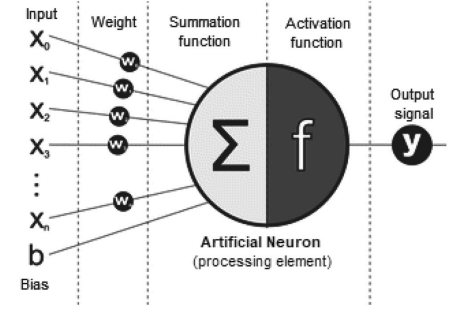
\includegraphics[scale=0.5]{Gambar/ArtificialNeuron.png}
    \caption{Skema Neuron Imitasi} \shortcite{sarker2021deep}
    \label{fig:neuron-scheme}
\end{figure}.

\begin{equation}
    \label{neural}
    y_i(x_i;W_i, b_i) = f(W_i \bullet x_i +b_i)
\end{equation}

Komponen utama jaringan DL terletak pada bagaimana tiap unit neuron saling terkoneksi dalam bentuk \emph{Multi Layer Perceptron} (MLP). Hal ini ditunjukkan pada Gambar \ref{fig:MLP-layers}. Sebuah jaringan MLP tersusun atas satu lapisan input, satu lapisan output, dan sebanyak \(N-2\) lapisan tersembunyi. Lapisan tersembunyi berfungsi sebagai lapisan komputasi yang tersusun atas sejumlah unit neuron dengan fungsi aktivasi untuk memproses data. Kedalaman dari MLP didefinisikan atas banyaknya lapisan tersembunyi sistem untuk mempelajari aspek tertentu dalam data. Akan tetapi, semakin banyak lapisan tersembunyi yang dimiliki model, model MLP dapat menjadi lebih sensitif dan rentan terhadap \emph{overfitting} \shortcite{murtagh1991mlp}.

\begin{figure}[htbp]
    \centering
    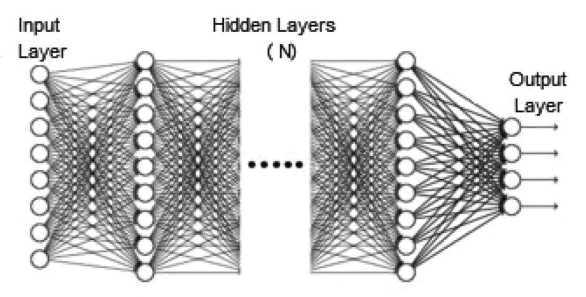
\includegraphics[scale=0.5]{Gambar/MultiLayerPerceptron.png}
    \caption{\emph{Multi Layer Perceptron}} \shortcite{sarker2021deep}
    \label{fig:MLP-layers}
\end{figure}

Konvergensi pemrosesan data jaringan MLP didapatkan melalui proses optimasi bobot dan bias melalui propagasi balik. Metode ini memungkinkan neuron untuk mempelajari karakteristik relevan dalam data dan menghasilkan output yang diharapkan berdasarkan fungsi biaya (\emph{cost function}) model. Fungsi biaya mengatur seberapa besar perbedaan prediksi model dengan target output. Bobot model diperbarui melalui proses minimalisasi nilai fungsi biaya terhadap bobot model secara iteratif \shortcite{shreshta2019AI}.

Proses optimasi bobot MLP dilakukan menggunakan algoritma \emph{gradient descent}. Bobot jaringan neural \(\theta\) diperbarui pada setiap iterasi dengan arah yang berlawanan terhadap gradien dari fungsi biaya, \(\nabla_\theta J(\theta)\). Ukuran besarnya pembaruan bobot dinyatakan oleh laju pembelajaran \(\eta\). Semakin kecil nilai \(\eta\), model belajar lebih lambat, tetapi semakin besar nilai \(\eta\), model rentan mengalami osilasi sehingga tidak mampu mencapai konvergensi \shortcite{ruder2016overview}. Metode \emph{gradient descent} dapat secara matematis dinyatakan dalam persamaan \eqref{grad-descent}. Berbagai metode turunan dari \emph{gradient descent} telah dikembangkan untuk meningkatkan efisiensi proses optimasi, seperti \emph{stochastic gradient descent} (SGD), \emph{adaptive moment-estimation} (ADAM), \emph{Limited-memory Broyden–Fletcher–Goldfarb–Shanno} (L-BFGS), maupun lainnya. 

\begin{equation}
    \label{grad-descent}
    \theta = \theta-\eta \nabla_\theta J(\theta; x^i;y^i)
\end{equation}

Normalisasi data perlu dilakukan selama proses optimasi untuk menjaga stabilitas dan efisiensi penurunan gradien. Normalisasi merupakan proses transformasi data dengan tetap menjaga sifat statistik data. Proses ini mengurangi perbedaan magnitudo fitur sehingga menyeimbangkan distribusi statistik gradien MLP. Dengan demikian, data dalam proses optimasi dapat terstruktur dengan baik tanpa menghambat kinerja model \shortcite{huang2023normalization}.

Pendekatan berbasis data dalam perambatan pulsa serat optik telah ditunjukkan dalam beberapa penelitian. Sebagai contoh, penggunaan jaringan konvolusi (\emph{Convolution Neural Network}/CNN) dalam menangkap perambatan sistem NLS dalam amplifier parametrik serat optik \shortcite{Sui:21}, maupun penggunaan jaringan \emph{Bidirectional Long Short-Term Memory} (Bi-LSTM) untuk memodelkan perambatan pulsa \emph{ultrashort} \shortcite{MARTINS2024103636}. Akan tetapi, metode berbasis data memiliki kelemahan atas dibutuhkannya dataset dalam jumlah besar supaya model dapat melakukan inferensi secara optimal. Selain itu, metode ini juga mengabaikan prinsip fisis yang terdapat pada tiap kasus \shortcite{wang2022applications}.

\section{Physics-Informed Neural Networks}

\emph{Physics-Informed Neural Networks} (PINNs) merupakan jaringan neural terspesialisasi untuk menyelesaikan kasus fisis \shortcite{raissi2019physics}. Hal ini dilakukan melalui modifikasi sistem jejaring neural melalui integrasi persamaan diferensial sistem (\emph{governing equation}) bersama batasan fisis seperti syarat awal dan syarat batas pada fungsi biaya model. Arsitektur PINNs diberikan pada Gambar \ref{Architecture}

\newpage
\begin{figure}[htbp]
    \centering
    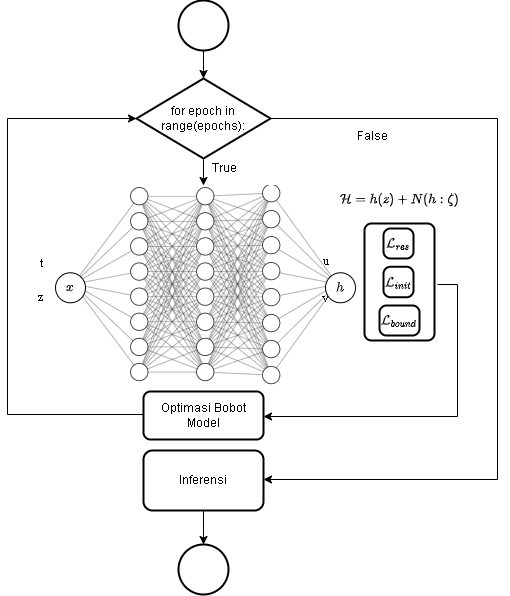
\includegraphics[width=0.6\linewidth]{Gambar/PINN.png}
    \caption{Arsitektur PINNs}
    \label{Architecture}
\end{figure}

Sebuah model PINNs digunakan untuk menyelesaikan sebuah sistem fisis yang diberikan pada persamaan diferensial \(\mathcal{H} = h(x) +N[h: \zeta] = 0\). Model ini menerima titik sampel $x$ sepanjang domain sistem, selanjutnya disebut sebagai titik kolokasi. Lapisan komputasi melakukan perhitungan untuk menghasilkan prediksi solusi persamaan diferensial $h$. Dari perhitungan ini, ditentukan nilai fungsi biaya. Diberikan tiga fungsi biaya pada sistem berupa fungsi biaya residu, $\mathcal{L}_{res}$, fungsi biaya syarat awal $\mathcal{L}_{init}$, dan fungsi biaya syarat batas $\mathcal{L}_{bound}$. Fungsi biaya residu diberikan berdasarkan persamaan diferensial $\mathcal{H}$. Fungsi biaya syarat awal dan fungsi biaya syarat batas didasarkan atas data kondisi awal dan kondisi batas yang diberikan.

\begin{equation}
    \label{residual-loss-func}
    \mathcal{L}_{res} = \frac{1}{N}\sum_{i=1}^N\mathcal{H}^2(x)
\end{equation}

\begin{equation}
    \label{initial-loss-func}
    \mathcal{L}_{init} = \frac{1}{N}\sum_{i=1}^N|h_{init} - \bar{h}_{init}|^2
\end{equation}

\begin{equation}
    \label{boundary-loss-func}
    \mathcal{L}_{init} = \frac{1}{N}\sum_{i=1}^N|h_{bound} - \bar{h}_{bound}|^2
\end{equation}

\noindent
Di mana $\bar{h}$ dan $h$ pada persamaan \eqref{initial-loss-func} dan \eqref{boundary-loss-func} masing-masing menyatakan solusi persamaan yang diketahui dan tebakan solusi persamaan oleh PINNs. Keseluruhan proses ini terus diulangi sehingga mencapai jumlah iterasi (\emph{epochs}) tertentu atau hingga didapatkan hasil yang konvergen. \shortcite{raissi2019physics}. 

Proses Optimasi PINNs dapat dilakukan menggunakan algoritma optimasi ADAM-LBFGS, yaitu perpaduan antara metode optimisasi berbasis \emph{stochastic gradient}, \emph{Adaptive Momentum Estimation} (ADAM) dan pendekatan quasi-Newton, \emph{Limited Memory Broyden–Fletcher–Goldfarb–Shanno} (L-BFGS). Strategi ini umum digunakan guna menawarkan konvergensi yang lebih cepat dan efisiensi komputasi yang tinggi. Performa model umumnya meningkat seiring dengan bertambahnya ukuran sampel dan jumlah epoch pelatihan. Sebaliknya, metode stochastic gradient descent (SGD) murni menghadapi keterbatasan dalam pengelolaan titik kolokasi pada sistem berdimensi tinggi \shortcite{cuomo2022scientific}.

Inisialisasi titik kolokasi model umumnya dilakukan dengan metode \emph{uniform random sampling}, \emph{latin hypercube sampling}, maupun \emph{sobol sequences} \shortcite{pangFPINNN}. Akan tetapi, selama pembelajaran, model mungkin mengalami kesulitan mencapai konvergensi pada daerah tertentu dengan karakteristik fisis yang lebih kompleks \cite{LiuAdapt}. Dengan demikian, pemilihan sampel domain tersebut tidak dapat menyelesaikan masalah ini seorang diri. Maka dari itu, dibutuhkan metode adaptif yang mampu memfokuskan kemampuan komputasi sistem pada daerah yang kesulitan dicapai model. 

\section{Synthetic Minority Over-sampling Technique}

SMOTE (\emph{Synthetic Minority Over-sampling Technique}) merupakan metode yang dirancang untuk mengatasi ketidakseimbangan dataset dalam fungsi klasifikasi. Metode ini bekerja dengan menginterpolasi data sintesis baru antara sebuah titik dan tetangga terdekat, \emph{K-Nearest Neighbor} dalam kelas data minoritas \shortcite{chawla2002smote}. SMOTE telah diaplikasikan dalam berbagai domain dalam fungsi klasifikasi, seperti deteksi penipuan, diagnosis penyakit, maupun pemrosesan sinyal. Kendati metode ini mampu meningkatkan performa klasifikasi, SMOTE berpotensi memberikan distribusi yang menyimpang dari distribusi sebenarnya pada data berdimensi tinggi maupun pada sampel minoritas yang terbatas \shortcite{ELREEDY201932}.